

\begin{frame}{Reprenons le schéma de la base des voyageurs}

Supposons qu'on ait validé la modélisation suivante
\vfill

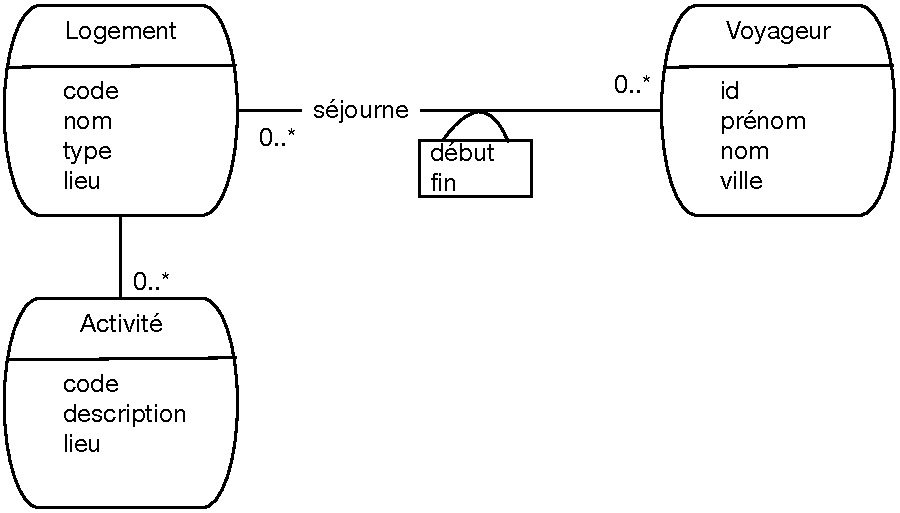
\includegraphics[width=8cm]{../figures-sql/schema-voyageurs}

\vfill

Il n'y a plus qu'à appliquer la normalisation.
\end{frame}


%%%%%%%%%%%%
\begin{frame}{Algorithme de normalisation}


\begin{redbullet}
  \item  Une entité définit une DF 
    de l'identifiant vers les attributs
    $$codeLogement \to nom, type, lieu$$
        
  \item Une association plusieurs-à-un définit une DF 
    entre les identifiants\,; la partie droite est une \alert{clé étrangère}
       $$codeActivit\acute{e} \to codelogement$$

  \item Une association plusieurs-à-plusieurs définit une clé et 
    une DF  entre cette clé et les attributs
    
    $$(codelogement, idVoyageur) \to d\acute{e}but, fin$$
\end{redbullet}


\vfill
\alert{C'est tout!}
\end{frame}

%%%%%%%%%%%%
\begin{frame}{Résultat pour la base des voyageyrs}

Clés primaires en \textbf{gras}, clés étrangères en \textit{italiques}.

\vfill
\begin{redbullet}
  \item Logement (\textbf{codeLogement},  nom, type, lieu)
  \item Activité (\textbf{codeActivité}, \textit{codeLogement}, description)
    \item Voyageur (\textbf{idVoyageur}, prénom, nom)
   \item Séjour (\textbf{\textit{idVoyageur}, \textit{codeLogement}}, début, fin)
\end{redbullet}


\vfill
NB: le nommage des attributs est libre.
\end{frame}


\begin{frame}{Versions améliorée (?)}

On a représenté Activité comme une entité faible, et Séjour comme une entité.
\vfill

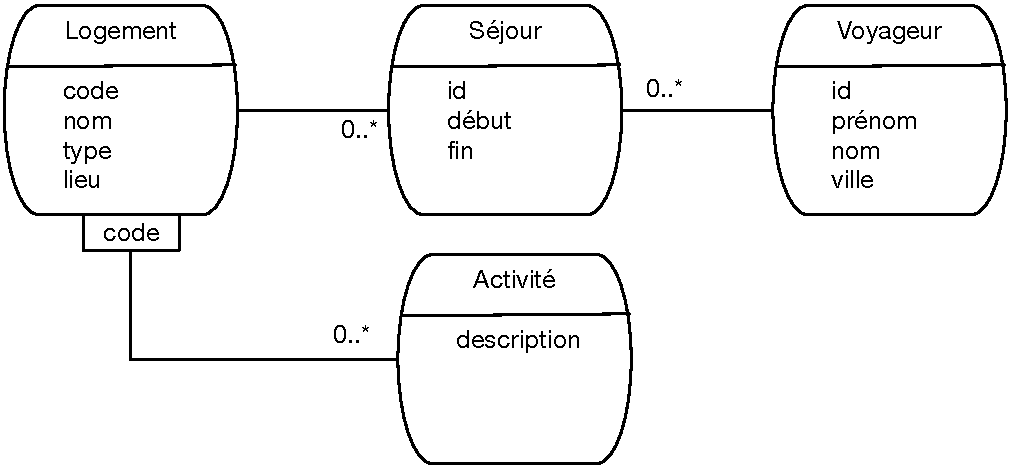
\includegraphics[width=7.5cm]{../figures-sql/schema-voyageurs-mieux}

\vfill

\begin{redbullet}
  \item Activité (\textbf{\textit{codeLogement},codeActivité}, description)
   \item Séjour (\textbf{idSéjour}, \textit{idVoyageur}, \textit{idLogement}, début, fin)
\end{redbullet}
\end{frame}

%%%%%%%%%%%%
\begin{frame}{Petit exemple}


\begin{small}
\begin{center}
\begin{minipage}[b]{4cm}
\begin{tabular}{c|c|c}
\textbf{code} & \textbf{nom} & \textbf{lieu}\\ \hline 
ca & Causses & Cévennes\\ \hline 
ge & Génépi & Alpes\\ \hline 
pi & U Pinzutu & Corse\\ \hline 
ta & Tabriz & Bretagne\\ \hline 
\end{tabular}
\centerline{La table \tble{Logement}}
\end{minipage} \hspace*{1cm} \
\begin{minipage}[b]{4cm}
\begin{tabular}{c|c|c}
\textbf{idV.} & \textbf{nom} & \textbf{prénom}\\ \hline 
10 & Fogg & Phileas\\ \hline 
20 & Bouvier & Nicolas\\ \hline 
30 & David-Néel & Alexandra\\ \hline 
40 & Stevenson & Robert Louis\\ \hline 
\end{tabular}
\centerline{La table \tble{Voyageur}}
\end{minipage} 
\end{center}
\begin{center}
\begin{tabular}{c|c|c|c|c}
\textbf{idSéjour} & \textbf{idVoyageur} & \textbf{codeLogement} & \textbf{début} & \textbf{fin}\\ \hline 
1 & 10 & pi & 20 & 20\\ \hline 
2 & 20 & ta & 21 & 22\\ \hline 
3 & 30 & ge & 2 & 3\\ \hline 
\end{tabular}
\centerline{La table \tble{Séjour}}
\end{center}
\end{small}
\end{frame}


%%%%%%%%%%%%%
\begin{frame}{À retenir}
À partir du schéma E/A, on applique l'algorithme de normalisation et on obtient
un schéma relationnel en 3FN.

\vfill

\begin{redbullet}
   \item Pas de magie: le schéma ne sera pas meilleur que la conception
   \item Attention à ne pas ``cacher'' de dépendance fonctionnelle dans une entité
   \item On peut ajouter des contraintes, typages et contrôles quand on crée les tables
\end{redbullet}

\vfill

Cf. le support de cours pour quelques compléments
\end{frame}

